\documentclass[12 pt]{article}
\renewcommand{\baselinestretch}{1}
\usepackage{geometry}
\usepackage{graphics}
\geometry{verbose,letterpaper,tmargin=0.5 cm,bmargin=0.8 cm,lmargin=2.5cm,rmargin=2.5cm,headsep=1cm}
\setlength{\parskip}{\smallskipamount}
\setlength{\parindent}{10 pt}
\usepackage{amssymb}
\usepackage{amsmath}
\usepackage{textcomp}
\usepackage{setspace}
\usepackage{indentfirst}
\usepackage{hyperref}

\usepackage{algorithm}% http://ctan.org/pkg/algorithms
\usepackage{algpseudocode}% http://ctan.org/pkg/algorithmicx
\usepackage{listings}
\usepackage{hyperref}
\usepackage{enumitem}
\usepackage{array}
\usepackage{tikz}
\usepackage{graphics}
\usepackage{standalone}
\usepackage{amsthm}
\usepackage{breakcites}
\title{Predictive analytics with online change detection in data streams}
\date{}
\begin{document}
	\maketitle
  \section{Summary}
  % summary 
  In batch, or, offline training settings, models are trained using a fixed training data set and then used to make predictions on incoming data. 
  However, streaming, or, on-line settings, are more prevalent in real world applications. 
  In both cases a concept drift can happen and the model performance can drop. 
  In order to detect concept drifts, change detectors are used to monitor changes in models performance metrics on-line~\cite{gama2004learning}. 
  Once change is alarmed the model can be re-trained using the most relevant data between last change point and current time moment.
  In this scenario model will be trained using only most recent relevant data batch and will have a better performance than sliding window or growing window updated model.

  In addition, we propose to use recurrency property to skip false alarms and possibly detect changes with smaller delays.

  Questions.
  If there is outlier and we make a prediction, then what is the correct prediction?
  If there is outlier and change is alarmed then it is considered as a change and situation is the same as depicted on Figure..
  If we change is not alarmed by having outlier, ...

  % sections
  There are various types of change detectors. 
  Section X describes concept drift phenomenon.
  Sections X,Y,Z describe Adwin, Cusum, Bayesian, etc.detectors.
  Section X describes recurrency property.
  Section X describes Pccf and its applications.
  Section XXX describes how recurrency helps to reduce FA rate and decrease detection delay for CFB signal.

  % figures
  Figure XXX illustrates concept drift phenomena when SVM model is applied in streaming settings to the Sine1 dataset. 
  Before concept drift error rate decreases according to the statistical decision theory cite{XXX} as model is adaptively retrained. 
  Performance drops after time moment $t$ and detectors alarms the change at the moment $t_1$. 
  Once retrained using relevant data between $t$ and $t_1$, performance becomes better than when updating model continuously.

  Figure XXX shows the decision boundary before and after concept drift in Sine1 dataset.

  Figure XXX illustrates an example of adaptive learning with detector and without. 
  It can be seen that with detector performance is better and with recurrent detector it is even more better because we can skip possible FA and we can possibly reduce the detection delay.

  In~\cite{SouzaRMB20}: One of the main problems is un uncertainty about the presence of concept drifts.

  Sliding window is a common approach.
  Figure~\cite{fig:art_sig_example} illustrates concept drift phenomenon when linear regression model is applied to artificially generated signal using sliding window approach. 
  The figure shows predictions and prediction errors.
  \begin{figure}[!htb]
    \centering
    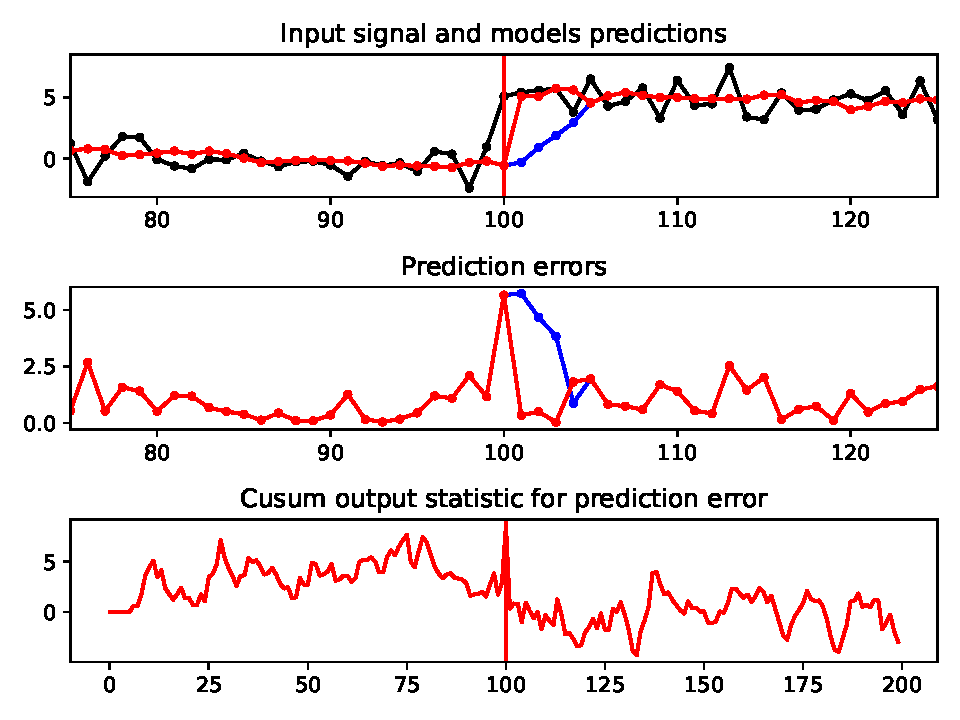
\includegraphics[width=0.7\textwidth]{images/proof_of_concept_linreg_art_sig}
    \caption{Artificial signal. Linear regression.}\label{fig:art_sig_example}
  \end{figure}

  Figure~\ref{fig:sine1_example}
  \begin{figure}[!htb]
    \centering
    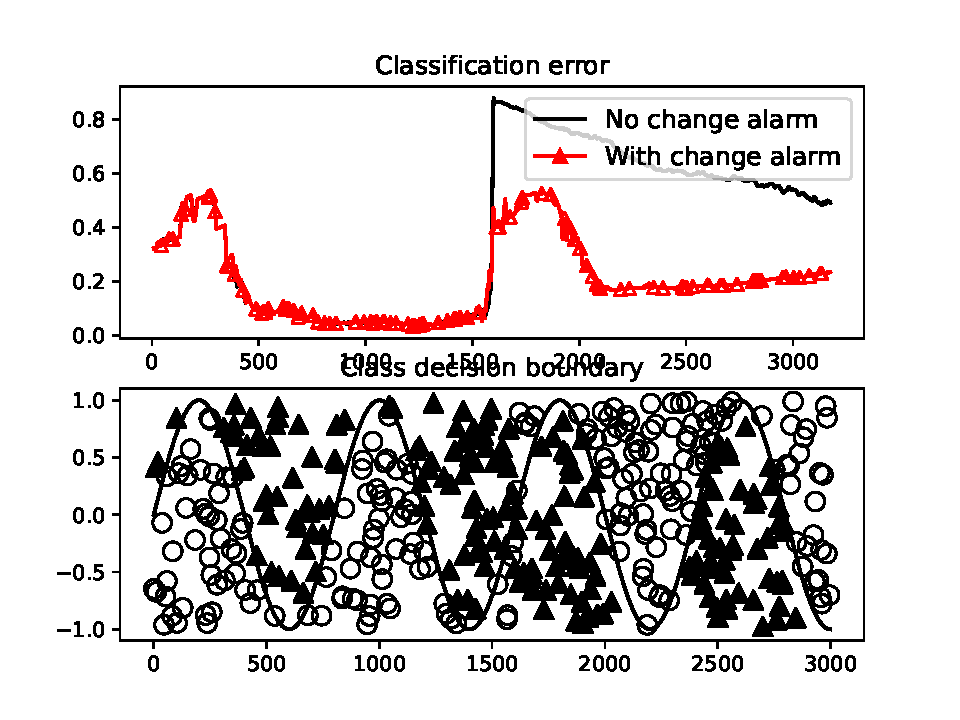
\includegraphics[width=0.7\textwidth]{images/proof_of_concept_dt_sine1}
    \caption{Artificial signal SINE1. Classification.}\label{fig:sine1_example}
  \end{figure}


  \bibliographystyle{unsrt}
  \bibliography{references}
\end{document}
